\documentclass{article}
\usepackage[utf8]{inputenc}

\title{CCLtracker Framework: Monitoring users learning and activity in web based citizen science projects
}
\author{ Jose Luis Fernandez-Marquez, Ioannis Charalampidis,\\ Oula Abu-Amsha, Francois Grey, Brian Fuchs, \\ Daniel K. Schneider, Ben Segal, S.P. Mohanty, Egle Marija Ramanauskaite}
\date{July 2015}

\usepackage{natbib}
\usepackage{graphicx}

\begin{document}

\maketitle

\begin{abstract}
The explosion of web applications and on-line services over the last 20 years have made analytics tools highly required to understand who the users are, how they find the web, and how they behave. That allows to monitor key performance indicators (e.g. downloads, sells, or participation on the web), improve users interfaces, plan, execute, and evaluate actions to increase users engagement. 

Measuring and improving users engagement in citizen science projects is not different than many other industrial applications such as on-line shopping, newspapers, or sites for recommending music or movies. However, citizen science project usually lack of resources for implementing a proper user monitoring system. Mainly, because there are not any tool providing a high-level API for implementing user monitoring in a reusable and modular way, thus requiring a huge development effort.  

This paper presents CCLTracker analytics framework to ease and overcome current analytics tool limitations, and providing an API for monitoring users activities such as time spent watching a video, time to do a task, or \% of page scrolled down. Additionally, the CCLTracker has been integrated in 3 different citizen science projects proving its usage for measuring learning. 

\end{abstract}

\section{Introduction}

% \begin{itemize}
%     \item  Why web tracking exist? (motivation)
%     \item  Relation between web tracking for commercial applications and non-profit and citizen science projects. 
%     \item Why existing tools are not satisfying our requirements? (2 paragraphs summarizing the related work and explaining the lack of tools like CCL tracker. 
%     \item Impact. 
% \end{itemize}



The explosion of web applications and on-line services over the last 20 years have made analytics tools highly required to understand who the users are, how they find the web, and how they behave. That allows to monitor key performance indicators (e.g. downloads, sells, or participation on web), improve users interfaces, planing, execute, and evaluate actions to increase users engagement. 

There are a bunch of different analytics tools such as Google Analytics, and Piwik, which provide very interesting analytics information about the users, and the website. These tools store and aggregate the analytics data, and provide a Graphical User Interface (GUI) that allows users without programming skills to manipulate analytics data and create customs reports to periodically monitor key performance indicators.  

However, the information regarding the user behaviour is limited to average time per session, pages views, or bound rate (i.e. percentage of people that leave the site without ant interaction). Both tools, GA and Piwik allows to send application specific events, i.e. events designed to be fired from your website when tracking specific actions. 

 For example, we can add number of click per sessions, number of times an user writes on the forum, clicks to internal and external links, whether the user is scrolling down the web or how long time an user has been watching a video. All these examples require to program a tracking system in the client side and connect it with the analytics tool. This tracking system is tough to implement and keep it updated over the different version of the web. Additionally, it creates dependencies with the analytics tools.

% which already have their own eco-system of services giving support and extending their functionality (i.e. Google Tag Manager, Google Query Explorer, visualization tools, Libraries to export data to programing languages, etc.).

This paper presents CCLTracker analytics framework to ease and overcome current analytics tool limitations. The main contribution of this framework is a Java Script library that can be easily connected to other analytics tools, providing:

\begin{itemize}
\item Client side aggregation of data before sending it to the analytics tool (i.e. GA or Piwik). 
\item High level API to ease the creation and manipulation of events. 
\item Decoupling between the tracking system and the analytics tools. I.e. Event created from CCLTracker library can be sent to Google Analytics, Piwik or whatever analytics tool able to capture JS events. 
\end{itemize}


As a proof of concept this paper shows the CCLTracker analytics framework composed of Google Analytics, Google Tag Manager, and the CCLtracker JS library. We present detailed results from a case study and show how the framework overcomes current Google Analytics limitations. 
 
Section~\ref{sec:related} describes existing analtyics tools and their limitations. Section~\ref{CCLTracker} introduces the CCLTracker framework. A case study is presented in Section~\ref{sec:caseStudy}. Finally we present conclusions and future work. 
 

\section{Background}\label{sec:related}


% \begin{itemize}
% \item Existing frameworks and tools for web user tracking (Google Analytics, piwik, and existing papers. For each of them advantages and disadvantages. 
% \item Tracking client side. There are many papers. 
% \item Basically this section should conclude highlighting the novelty of CCLTracker on the state of the art. 
% \end{itemize}
   
   
There are two main web-based analytics tools, Google Analytics~\cite{} and Piwik~\cite{}. A major difference between then is that Piwik is open source and you can deploy it in a local environment, having full control, full access to the data, and privacy. On the other hand Google analytics is a free service provided by google, and the information is stored in their servers. Additionally, Google Analytics provides demographic information about the users such as, age, gender and interests. Both analytics tools provide information about the users in three categories: audience, acquisition, and behaviour.

\textbf{Audience} provides information about who the users are, and general information about the site performance such as number of users, number of sessions, page views, or average pages per session. Regarding the users we can gather information about their age, gender, location, their interest (affinity category and in-market segment), the browsers, mobile phones, operating systems, screen resolutions, or languages. 
   
\textbf{Acquisition} provides information about how the users reach the website. I.e. using the URL (direct), using a organic search, from a referral or social media. This information helps to evaluate dissemination activities.   

\textbf{Behaviour} provides information about what the user is doing in the website, e.g. pages visited, or behavior flow, and information about the site performance, e.g. Average page load time, or average server connection time. Additionally, this section provides information about user events. User events allow to track user activities within the website, but each of the events requires to be implemented in our website. Events are extremely important to understand what the user is doing in the website, everything can be tracked but it can involve a high complexity. E.g. Internal/external clicks, time spent between clicks, mouse trajectories, scroll down on the pages, time spent watching a video or listening an audio, etc. Events provide a very powerful tool for large scale debugging. Events can be user actions, but also system errors. Tracking system errors such as problem downloading a file, web service not available, or wrong email in the log in session, provide two main advantages. On one hand we can easily detect bugs that appear with very low frequency, i.e. 1/1000 or 1/10000. On the other hand, we can cross the information regarding the error with information coming from Google Analytics such as browser, Operative System, screen resolution, or Internet provider. Crossing those data, allows as to reproduce the errors and fix them using users as debuggers. Notice that this implementation requires an experienced programmer and it couples the website code with the analytic tool. It gets very tough to implement when we are using complex Java Script applications and it is difficult to maintain through out the application development cycles, i.e. little changes on the functional code of the application might make produce wrong analytics data.  

   
  
 
There are three major ways of manipulating data in GA: \textbf{Crossing, Segmenting and Filtering}. Google Analytics allows to cross data by adding a second dimension, e.g. we can see number of users per country, or number of session coming from Facebook per country. Segmentation allows us to focus the analytics data on a subset of sessions or users, e.g. users coming from Spain, new users, female users, users between 18 and 24 years old, users coming from Reddit. Filtering allows to clean the data and remove those that is not relevant. E.g. we could ask for all referrals order by bounce rate to know the user engagement from different referrals, however, we can find at the top referrals with few users that are not relevant for the stats. In this case we can apply a filter to remove from the list those referrals with less than a number of users. 



An interesting feature provide by GA is \textbf{Custom Reports}. Custom reports allow to create templates with aggregated data, applying crossing, segmentation and filtering. Custom reports are used to periodically monitor key performance indicators saving time on creating the aggregations. 


\subsection{Current limitations}

There two types of limitations in GA: limitations regarding data limits\footnote{https://support.google.com/analytics/answer/1070983?hl=en}, such as 10 million hits per month or 200,000 sessions per day. Those limitations maybe skipped by upgrading to Google Analytics Premium which has an associated cost, or using another analytic tools such as Piwik which is open source and there are not data limits. Notice that Piwik does not provide analytics data about the users' age, gender, or interest. Moreover, Piwik requires to be hosted and managed in our own servers. 

The second type of limitations refer to functional limitations. Most of existing limitations can be overcome by using external tools. For example, it is not possible to do cluster analysis or user profiling in GA. However, there are libraries for exporting data to R~\cite{} or services to export data in standard format such as Google Query Explorer\footnote{https://ga-dev-tools.appspot.com/query-explorer/}. Moreover, it is not possible to make analytics data public because the access to GA data requires authentication, in this case we can user Google Super Proxy\footnote{https://developers.google.com/analytics/solutions/google-analytics-super-proxy} which allow to create a proxy using your credential and provide the data using standard formats that can be visualised using APIs such as Google Charts\footnote{https://developers.google.com/chart/}.


One of the major limitations comes when we want to measure engagement or measuring some kind of user activity in our website. Information provided by GA regarding engagement is very poor, e.g. time per session, bounce rate, or pages views. For example an on-line shop would like to know about those people who buy, or those who leave the site without buying. In a citizen science project~\footnote{http://crowdcrafting.org/} it would be interesting who are the people contributing and who are those who visit the site but there are not participating, who are posting information on the forum, or who are playing a key role on the project. To get this data we need to use application specific events, i.e. events monitoring user activity on the web. In this case, developers need to implement it and release a new version of the site. Some times, specially in big companies, this new analytics requirements need to wait for the approval and the next official release. In order to mitigate this delay and make data scientist more independent from web developers, google released Google Tag Manager\footnote{http://www.google.com/tagmanager/} (GTM). GTM allows to add new tags (tracking new events) by using a graphical interface, and inject the code in the website without need to wait for developers to release the code. There many others tools and service that can be user to overcome limitations and extend GA functionality. That makes GA not a simply tool, but an eco-system of developers, tools, services, and users.

This paper aims to mitigate the complexity of adding application specific events (i.e. tracking events) and decouple the dependency with Google Analytics or any other tracking tool, allowing to migrate to other tracking tools or having the tracking data replicated in a local server. Many companies are using google analytics and integrated tags in their tracking code, i.e. where user click, when they manage to sell a product, user profiling, or tracking user attention, however, that involves a huge developing effort, and once it is implemented the tracking code will be coupled to the analytics tool. For example, if we are using GA and we reach the data limit we will find to option: pay for a premium account or send fewer hits to GA. Migrating to another analytics tools such as Piwik or storing the data in a local server will involve a huge developing effort. Additionally, as far as we know there is not any library focusing on mitigating this effort, by providing a high level API to ease the implementation of application specific events. 


% I am not sure if we should mention the problem of advance segmentation. 


In this paper we propose CCLTracker library which provides a high level API for tracking events and decouple your tracking code from any analytics tool, thus allowing to easily migrate to another existing analytics tool or to store the application specific events locally. CCLtracker library is implemented in Java Script and integrated in the CCLTracker Framework (See section~\ref{sec:CCLtrackerFramerwork}). The CCL tracking framework is composerd by GA, Google Tag Manager (GTM), Google Super Proxy, and the CCLTracker library (see section\ref{sec:CCLtrackerFramerwork} for more details). 


\subsection{Learning analytics (OULA)}
\begin{itemize}
\item Why to use analytics data for measuring learning?
\item References about learning analytics in CCS projects, also MOOC courses
\end{itemize}

 
\section{CCLTracker JS library (IOANNIS}

\begin{itemize}
\item What is CCLTracker JS library?
\item What is the contribution of using CCLTraker library compared with starting a implementation from scratch. 
\item Technical description of the Library
\item Setting up the library, requirements, scope,...

\end{itemize}


\section{CCLTracker Framework}\label{sec:CCLtrackerFramerwork}

The CCLTracker JS Library has been integrated in a framework composed by the following tools and services:

\textbf{Google Analytics (GA)} provides storage, aggregation and visualization of data. Additionally GA provides web based analytics information. Information about users activities and system performance is sent by Google Tag Manager. 

\textbf{Google Tag Manager (GTM)} is in charge of structuring the analytics data and send it to GA. GTM receives event generated by the CCLTracker Library that are fired from the website. GTM is used as connector between the website and the analytic tool (GA in this case). By changing GTM settings we could address another analitycs tool such as Piwik, or directly store the events in a local server without requiring any change on the website code. 

\textbf{Google Query Explorer} is used to retrieve analytics data from GA. The queries created in Google Query Explorer are used in R for advance aggregation and Google Super Proxy for making data publicly available. 

\textbf{R language} is used to created advance aggregation of analytics data. It allows us to measure engagement in many different ways, and using cluster algorithms for gather users profiles. 

\textbf{Google Super Proxy} allows us to make public analytics data, and share it with the website users. 


One of the major decisions taken in this framework was the use of GA. GA was adapted as analytics tools because the demographics information they provide, the fast set up time, it is a free service, and its strong community using it. 



\begin{figure}[t]
  \begin{center}
		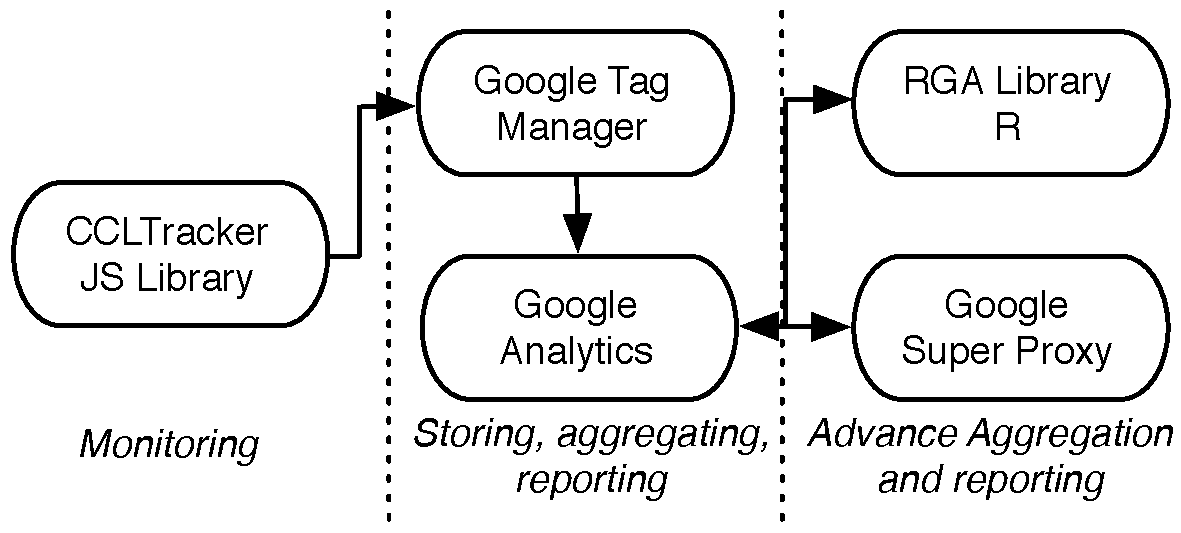
\includegraphics[width=11cm]{imgs/ccltrackerFramework.pdf}
  \end{center}
\caption{CCLTracker Framework Components}
\label{img:CCLTrackerFrameworkComponents}
\end{figure}

Figure~\ref{img:CCLTrackerFrameworkComponents} shows the interaction between the different components of the CCLTracker Framework. 


% Notice that there is not a dependency between the CCLTracker Library and GA. Events generated by the CCLTracker Library can be received from Google Tag Manager and sent to GA, or it can be received from GTM and send to Piwik, or it could be received from an external process and store the data in a local data base. 


\section{Proof of concept}

This section summarises the main applications where the CCLTracker framework has been used and show data examples. 

The CCLTracker framework has been implemented under the EU project Citizen CyberLab. The main goal was to evaluate the different pilots developed during the project, evaluate the engagement, dissemination actions, and evaluate learning aspect of the pilots.

CCLTracker framework has been implemented in the following pilots:

\begin{itemize}
\item \textbf{CERN Volunteer Computing Challenge}\footnote{https://test4theory.cern.ch/challenge/} is  web site running periodic public volunteer computing challenges. Volunteers help CERN scientists simulate particle collisions in accelerators like the Large Hadron Collider (LHC), using their own computers. Namely, there were two event CERN 60 public computing challenge in 2014 and CERN Public Computing Challenge in 2015. 

\item \textbf{GeoTag-X}\footnote{www.geotagx.org/} is a website focuses on crowdsource photo analysis for humanitarian disaster response.

\item \textbf{Virtual Atom Smasher}\footnote{http://test4theory.cern.ch/about/} is an educational interactive game that teaches users about particle physics, while in the same time helps theoretical physicists at CERN with their research.
\end{itemize}


The CCLTracker Framework has been integrated in these applications in order to understand the users behaviour, measuring engagement and users' learning. 


\subsection{CERN Volunteer Computing Challenges}

The CERN 60 Challenge was a 12-days event that run during the last days of December 2014 (9-20 Dec.). The purpose of the challenge was to test the experimental CernVM WebAPI technology and to understand the user behaviours in volunteering computing projects.

\subsubsection{Event forwarding specifications}

We are using Google Analytics for handing the analytics events, which is delivered through Google Tag Manager. The latter offers the ability to dynamically inject additional tracking logic at a later time. However due to the complexity of the processes involved, it’s frequently not easy to identify the events of interest from an external library. For instance, it might be easy to track clicks on the “Start” button, but it’s not easy to understand if this action really started the Virtual Machine.

Therefore we need to have a higher-level information that should come directly from the application. In order to accommodate future changes in the way the analytics data are processed, we agreed on an interface between the application developer and the analytics experts. 


\begin{figure}[t]
  \begin{center}
		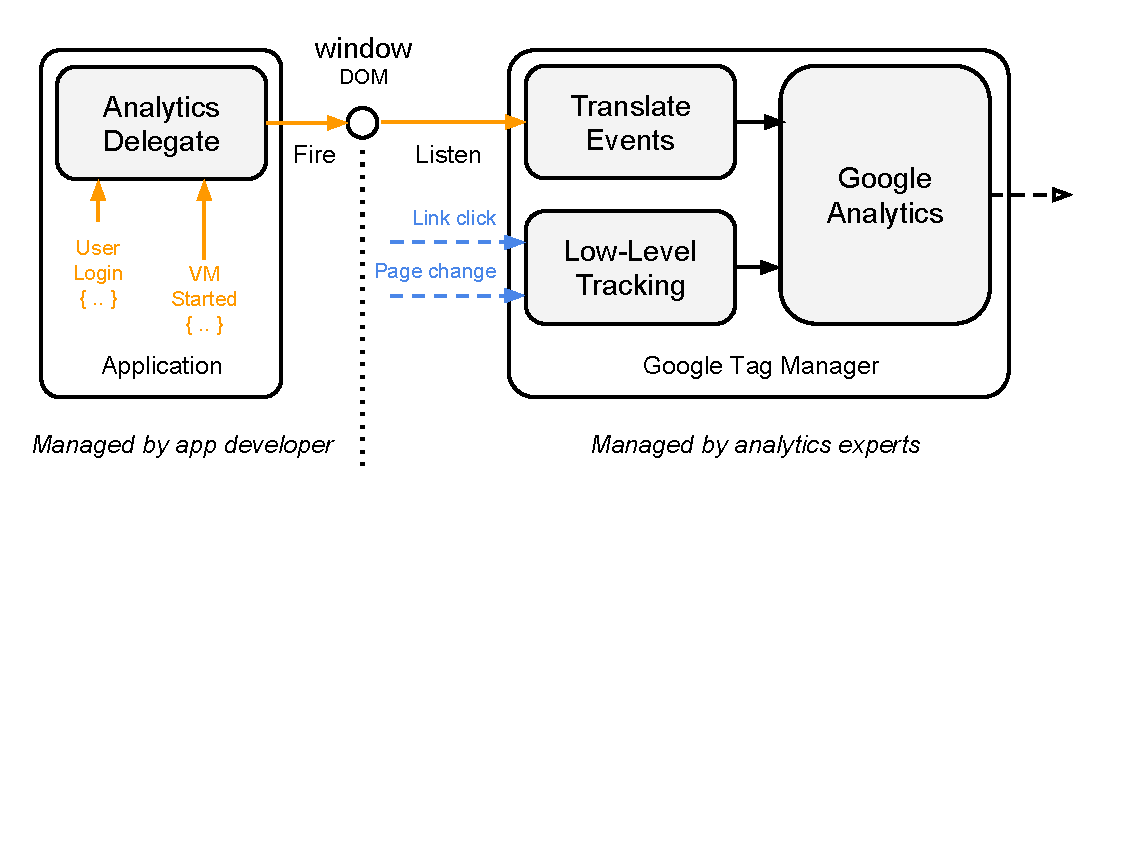
\includegraphics[width=\columnwidth]{imgs/CERN60Events.pdf}
  \end{center}
\caption{xxx}
\label{xxx}
\end{figure}



As seen in the above diagram, the application developer is triggering high-level events to an Analytics Delegate class. This class is then firing the appropriate events to the window DOM, not requiring anyone to listen for them.

When the analytics logic is managed by the analytics experts and is delivered via Google Tag Manager. It listens for analytics events in the window DOM, translates them to an appropriate format and forwards them to Google Analytics. The developer and the analytics experts maintain a document that lists all the possible events fired by the Analytics Delegate, along with the information each event carries. This way, they can optimally select and/or pre-process the high-level events into their preferred format.

In addition, the analytics experts can deliver extra, low-level tracking logic (for example listening for mouse clicks or page changes) that can provide them with additional information as required.

\subsubsection{Description of the events}

The tracking is implemented via high-level events fired by the Challenge interface, which are then collected and forwarded to the Google Analytics. There are two major categories of events:

Related to CernVM WebAPI 
Related to user actions

The events fired to the DOM window are always prefixed with the ‘analytics.’ prefix.

\subsubsection{CernVM WebAPI Events}

Most of the CernVM WebAPI events are fired when the state of the internal finite-state-machine is changed. For reference, the following abstract diagram illustrates the different states in the internal FSM and the possible transitions between them:



\begin{figure}[t]
  \begin{center}
		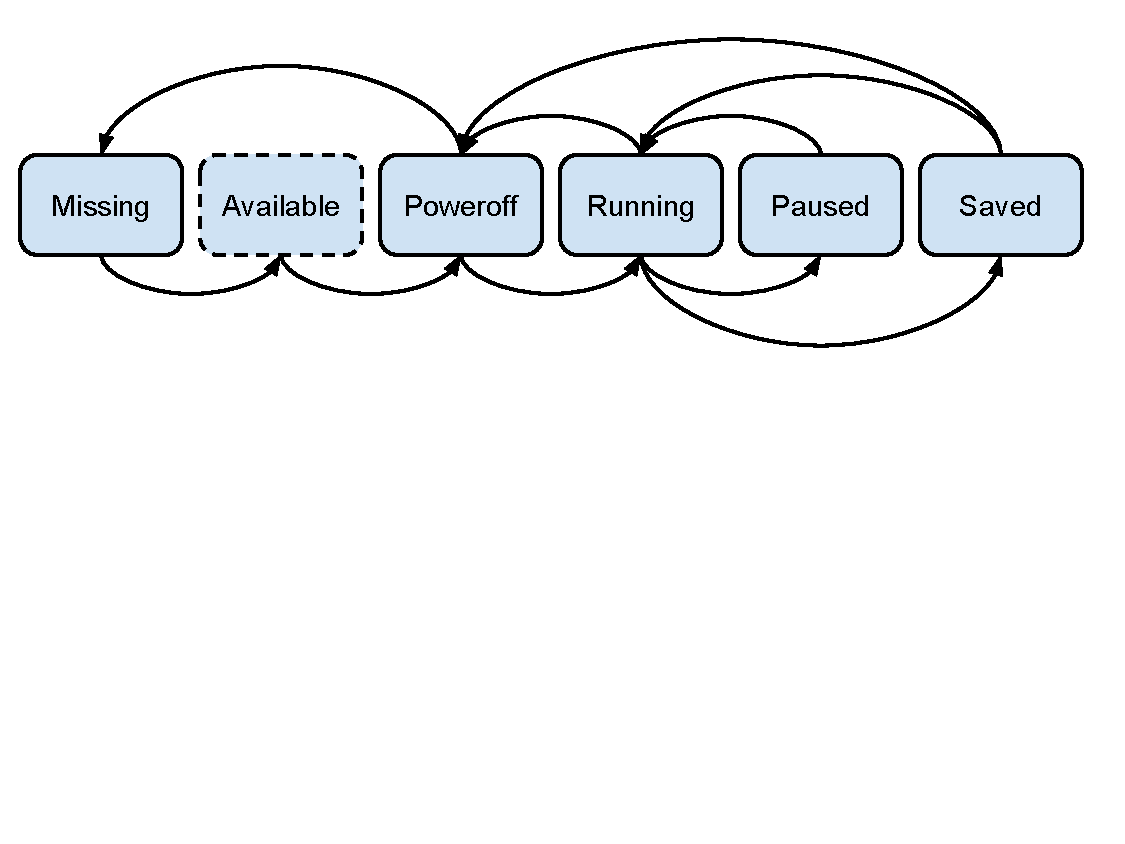
\includegraphics[width=\columnwidth]{imgs/webAPIEvents.pdf}
  \end{center}
\caption{xxx}
\label{xxx}
\end{figure}


When the path of actions is completed and the FSM settles on a target state, the following events are fired:

\begin{itemize}
    \item {\bf vm.missing}: the VM does not exist.
    \item {\bf vm.available}: the VM is defined in virtualbox but not yet configured.
    \item {\bf vm.poweroff}: The VM is properly configured and powered off.
    \item {\bf vm.saved}: the VM process has stopped and the state is saved to disk (hibernation)"
    \item {\bf vm.paused}: the VM process is running yet it’s CPU is halted (paused in-memory).
    \item {\bf vm.running}: the VM is running.
\end{itemize}

In addition, two special events are fired providing a higher-level information regarding the application that runs inside the Virtual Machine:

\begin{itemize}
\item {\bf vm.booted}: this event is fired when WebAPI fires the callback apiStateChanged(true), meaning that the designated port which is used for API communication between the javascript interface and the VM is available. We are assuming that the VM is “booted” because the port will be opened after the boot sequence is completed.

{\textit NOTICE: This event might oscillate, because changes in the network connectivity (ex. user closing the laptop lid) will interrupt the communication, causing this event to be fired again when the network connectivity is resumed.}

\item {\bf vm.collisions}: when through the API port, the javascript interface identifies that collisions are happening.

{\textit NOTICE: This event has similar oscillations to vm.booted. That’s because the javascript interface is probing the job status through the API port. If the API port becomes unavailable, the interface will assume that there are no more jobs being processed. Therefore the instant it becomes available again (vm.booted), this event will be fired again.}

\end{itemize}


\subsubsection{Sequence of events}

Since all these events are produced by the state changes of the FSM, they can only appear in sequences. The usual flow of events is shown on the following diagram:

\begin{figure}[t]
  \begin{center}
		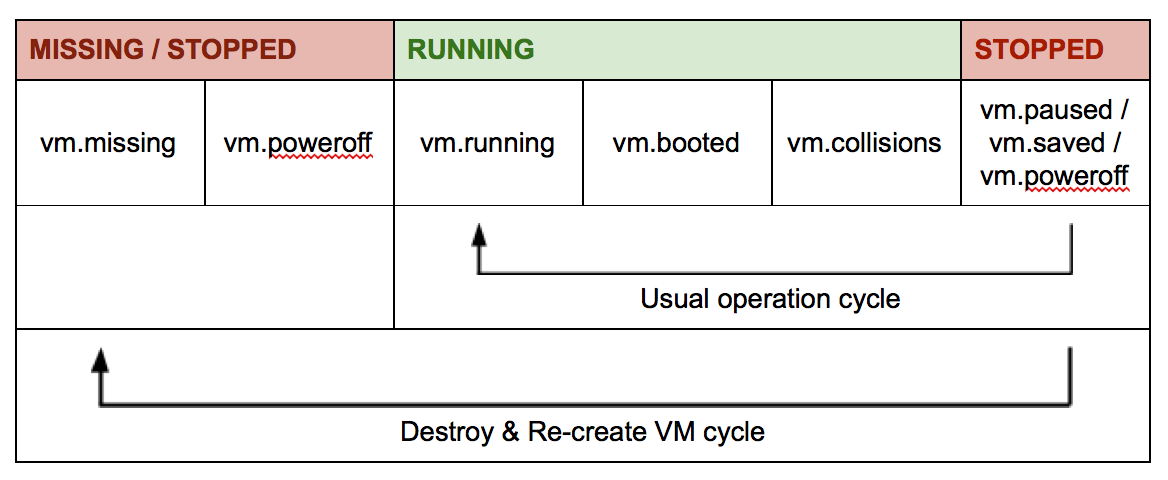
\includegraphics[width=\columnwidth]{imgs/sequenceOfEventsTable.png}
  \end{center}
\caption{xxx}
\label{xxx}
\end{figure}



Therefore, you can extract some useful information:

\begin{itemize}
\item {\bf How long the VM was running?}: sum the differences in timestamps between the event "vm.running" and ANY of the following three events: "vm.paused", "vm.saved", "vm.poweroff"

\item {\bf Did the user successfully manage to start a simulation?}: Check if AT LEAST one "vm.booted" event is fired after the “vm.running” event.
\end{itemize}


\subsubsection{User Events}

These events are fired by user actions on the user interface. These are:

\begin{itemize}
    \item {\bf actions.open\_rdp}: user clicked on the "eye" icon that opens the console window. There the user can see the status of the job and the job manager.
    
    \item {\bf actions.open\_web}: user clicked on the "pop-out" icon that opens the website served from within the Virtual Machine. There the user can see the histograms produced by the current simulation
actions.remove: User clicked on the trash icon which is going to remove the virtual machine from his/her computer.
    \item {\bf actions.start}: user clicked on the “start” button, which is going to create, set-up and boot the VM. If the VM is already in any other state it will be switched to ‘running’ by following the path in the FSM diagram.
    \item {\bf actions.stop}: user clicked on the “stop” button, which is going to SAVE the Virtual Machine to the disk (hibernate). 
    \item {\bf actions.apply}: user clicked on the “apply” button, which is going to apply the changes (s)he did on the CPU/RAM.
    \item {\bf actions.login}: user logged in with his/her social profile
    \item {\bf actions.logout}: user disconnected his/her social profile
\end{itemize}


\subsubsection{Sequence of events with WebAPI}

Most of the events fired by the WebAPI are triggered by the user. The following table shows which WebAPI events can a user event trigger. The events not included in the following table are not causing changes to the Virtual Machine.

If you notice a sequence of events not matching the ones below, then the state change of the VM was most probably triggered by an external cause. 


\begin{figure}[t]
  \begin{center}
		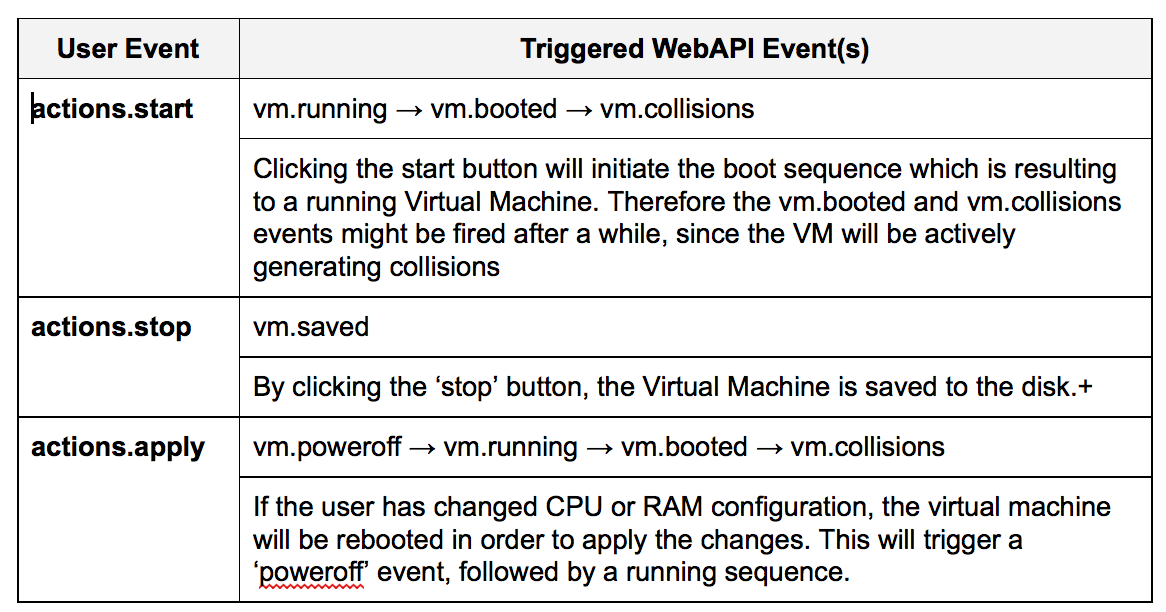
\includegraphics[width=\columnwidth]{imgs/webAPIEventsSequenceTable.png}
  \end{center}
\caption{xxx}
\label{xxx}
\end{figure}



\subsubsection{Other user actions that could trigger WebAPI events}

Since the user can still control the Virtual Machine without the Challenge Interface (ex. through VirtualBox), a state change can occur without a user-triggered action.


\begin{figure}[t]
  \begin{center}
		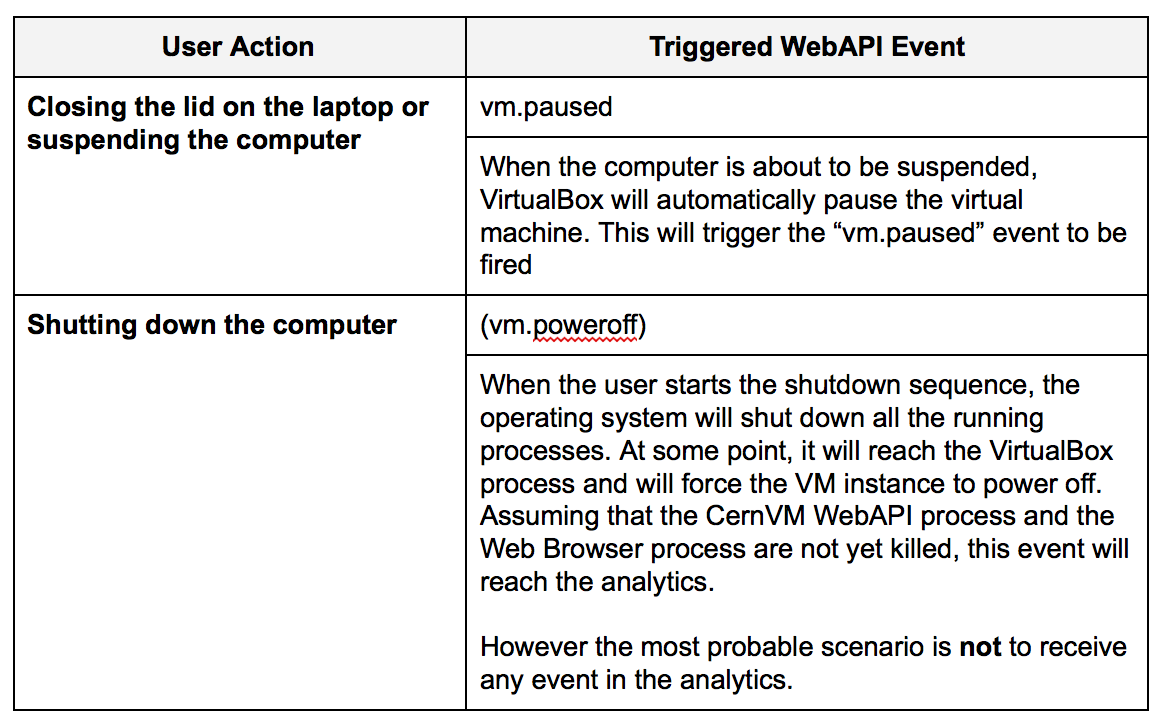
\includegraphics[width=\columnwidth]{imgs/userActions-webAPIEventsTable.png}
  \end{center}
\caption{xxx}
\label{xxx}
\end{figure}







% \begin{itemize}
% \item Briefly describe all projects using CCLtracker, Geotagx, VAS, 1st and 2nd CERN Challenges.
% \item Focus on CERN challenges showing some examples of the data we gathered. 

% \item It would be good to relate this data with the advantages we wrote in related work. 

%  e.g. debugging tools --> Trace of errors combined with browsers, OS, device, etc..
%       Knowing who are they --> Different segments and demographic information
      
%       Knowing their engagement --> picture about engagements. 
      
%       etc...

% \end{itemize}





\subsection{Data analysis}

This section shows results gathered from the CERN Volunteer Computing Challenge using the CCLTracker framework. 

Figure~\ref{img:Sessions versus sessions running the VM} shows the total number of sessions per day (blue line) compared with those sessions where the users execute the Virtual Machine (VM) (blue line), i.e. the user really participate in the challenge . 






\begin{figure*}[t]
  \begin{center}
		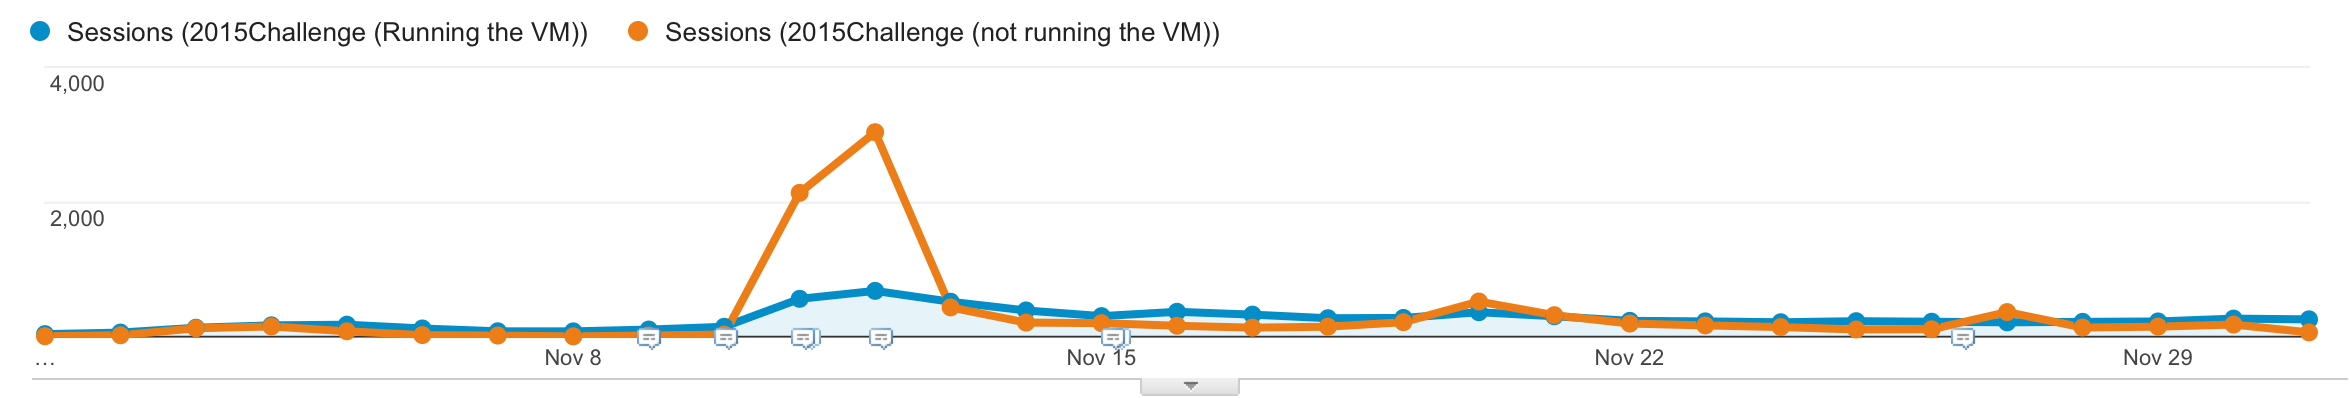
\includegraphics[width=15cm]{imgs/sessionVSsessionVMRunning.png}
  \end{center}
\caption{Sessions versus sessions running the VM}
\label{img:Sessions versus sessions running the VM}
\end{figure*}

      
    
    
    
      
      
\begin{figure}[t]
  \begin{center}
		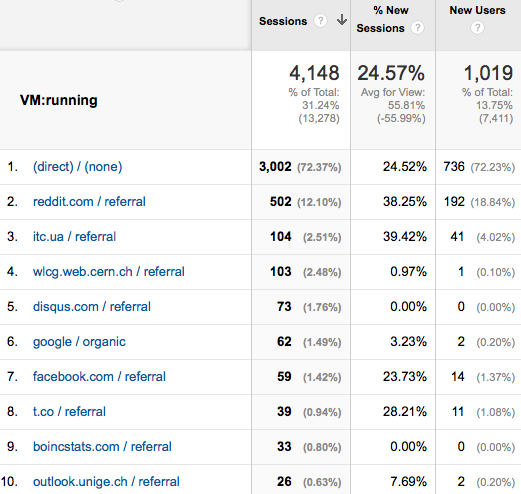
\includegraphics[width=\columnwidth]{imgs/sourceMediumVMRunning.png}
  \end{center}
\caption{Acquisition - Num. of sessions running VM by Source/Medium}
\label{img:AcquisitionRunningVM}
\end{figure}      
      
      


\begin{figure}[t]
  \begin{center}
		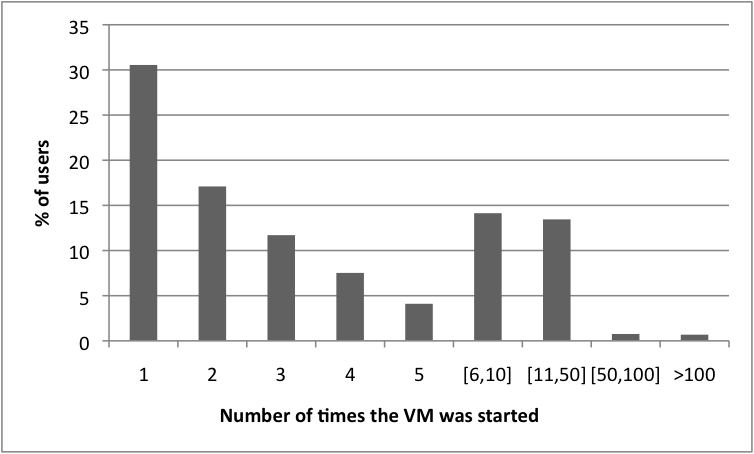
\includegraphics[width=\columnwidth]{imgs/Engagement.png}
  \end{center}
\caption{Engagement - number of times users are running the VM}
\label{img:EngagementVMrunning}
\end{figure}


\begin{figure}[t]
  \begin{center}
		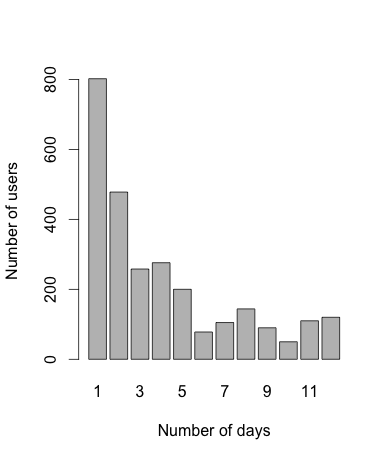
\includegraphics[width=\columnwidth]{imgs/Engagement2.png}
  \end{center}
\caption{Engagement - number of users/number of days}
\label{img:Engagement-days}
\end{figure}











\section{Conclusion}


\section{Future work}

\begin{itemize}
\item Setting up time/effort. 
\item Mix with contextual information. E.g. mobile phone data 
\item (we will find it out)
\end{itemize}



\bibliographystyle{plain}
\bibliography{references}
\end{document}
